\documentclass[1p]{elsarticle_modified}
%\bibliographystyle{elsarticle-num}

%\usepackage[colorlinks]{hyperref}
%\usepackage{abbrmath_seonhwa} %\Abb, \Ascr, \Acal ,\Abf, \Afrak
\usepackage{amsfonts}
\usepackage{amssymb}
\usepackage{amsmath}
\usepackage{amsthm}
\usepackage{scalefnt}
\usepackage{amsbsy}
\usepackage{kotex}
\usepackage{caption}
\usepackage{subfig}
\usepackage{color}
\usepackage{graphicx}
\usepackage{xcolor} %% white, black, red, green, blue, cyan, magenta, yellow
\usepackage{float}
\usepackage{setspace}
\usepackage{hyperref}

\usepackage{tikz}
\usetikzlibrary{arrows}

\usepackage{multirow}
\usepackage{array} % fixed length table
\usepackage{hhline}

%%%%%%%%%%%%%%%%%%%%%
\makeatletter
\renewcommand*\env@matrix[1][\arraystretch]{%
	\edef\arraystretch{#1}%
	\hskip -\arraycolsep
	\let\@ifnextchar\new@ifnextchar
	\array{*\c@MaxMatrixCols c}}
\makeatother %https://tex.stackexchange.com/questions/14071/how-can-i-increase-the-line-spacing-in-a-matrix
%%%%%%%%%%%%%%%

\usepackage[normalem]{ulem}

\newcommand{\msout}[1]{\ifmmode\text{\sout{\ensuremath{#1}}}\else\sout{#1}\fi}
%SOURCE: \msout is \stkout macro in https://tex.stackexchange.com/questions/20609/strikeout-in-math-mode

\newcommand{\cancel}[1]{
	\ifmmode
	{\color{red}\msout{#1}}
	\else
	{\color{red}\sout{#1}}
	\fi
}

\newcommand{\add}[1]{
	{\color{blue}\uwave{#1}}
}

\newcommand{\replace}[2]{
	\ifmmode
	{\color{red}\msout{#1}}{\color{blue}\uwave{#2}}
	\else
	{\color{red}\sout{#1}}{\color{blue}\uwave{#2}}
	\fi
}

\newcommand{\Sol}{\mathcal{S}} %segment
\newcommand{\D}{D} %diagram
\newcommand{\A}{\mathcal{A}} %arc


%%%%%%%%%%%%%%%%%%%%%%%%%%%%%5 test

\def\sl{\operatorname{\textup{SL}}(2,\Cbb)}
\def\psl{\operatorname{\textup{PSL}}(2,\Cbb)}
\def\quan{\mkern 1mu \triangleright \mkern 1mu}

\theoremstyle{definition}
\newtheorem{thm}{Theorem}[section]
\newtheorem{prop}[thm]{Proposition}
\newtheorem{lem}[thm]{Lemma}
\newtheorem{ques}[thm]{Question}
\newtheorem{cor}[thm]{Corollary}
\newtheorem{defn}[thm]{Definition}
\newtheorem{exam}[thm]{Example}
\newtheorem{rmk}[thm]{Remark}
\newtheorem{alg}[thm]{Algorithm}

\newcommand{\I}{\sqrt{-1}}
\begin{document}

%\begin{frontmatter}
%
%\title{Boundary parabolic representations of knots up to 8 crossings}
%
%%% Group authors per affiliation:
%\author{Yunhi Cho} 
%\address{Department of Mathematics, University of Seoul, Seoul, Korea}
%\ead{yhcho@uos.ac.kr}
%
%
%\author{Seonhwa Kim} %\fnref{s_kim}}
%\address{Center for Geometry and Physics, Institute for Basic Science, Pohang, 37673, Korea}
%\ead{ryeona17@ibs.re.kr}
%
%\author{Hyuk Kim}
%\address{Department of Mathematical Sciences, Seoul National University, Seoul 08826, Korea}
%\ead{hyukkim@snu.ac.kr}
%
%\author{Seokbeom Yoon}
%\address{Department of Mathematical Sciences, Seoul National University, Seoul, 08826,  Korea}
%\ead{sbyoon15@snu.ac.kr}
%
%\begin{abstract}
%We find all boundary parabolic representation of knots up to 8 crossings.
%
%\end{abstract}
%\begin{keyword}
%    \MSC[2010] 57M25 
%\end{keyword}
%
%\end{frontmatter}

%\linenumbers
%\tableofcontents
%
\newcommand\colored[1]{\textcolor{white}{\rule[-0.35ex]{0.8em}{1.4ex}}\kern-0.8em\color{red} #1}%
%\newcommand\colored[1]{\textcolor{white}{ #1}\kern-2.17ex	\textcolor{white}{ #1}\kern-1.81ex	\textcolor{white}{ #1}\kern-2.15ex\color{red}#1	}

{\Large $\underline{12a_{0462}~(K12a_{0462})}$}

\setlength{\tabcolsep}{10pt}
\renewcommand{\arraystretch}{1.6}
\vspace{1cm}\begin{tabular}{m{100pt}>{\centering\arraybackslash}m{274pt}}
\multirow{5}{120pt}{
	\centering
	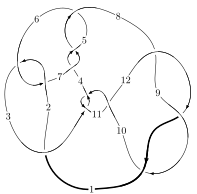
\includegraphics[width=112pt]{../../../GIT/diagram.site/Diagrams/png/1263_12a_0462.png}\\
\ \ \ A knot diagram\footnotemark}&
\allowdisplaybreaks
\textbf{Linearized knot diagam} \\
\cline{2-2}
 &
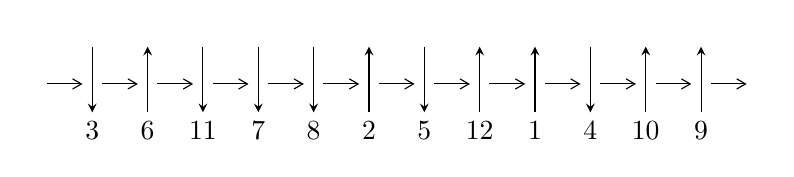
\begin{tikzpicture}[x=20pt, y=17pt]
	% nodes
	\node (C0) at (0, 0) {};
	\node (C1) at (1, 0) {};
	\node (C1U) at (1, +1) {};
	\node (C1D) at (1, -1) {3};

	\node (C2) at (2, 0) {};
	\node (C2U) at (2, +1) {};
	\node (C2D) at (2, -1) {6};

	\node (C3) at (3, 0) {};
	\node (C3U) at (3, +1) {};
	\node (C3D) at (3, -1) {11};

	\node (C4) at (4, 0) {};
	\node (C4U) at (4, +1) {};
	\node (C4D) at (4, -1) {7};

	\node (C5) at (5, 0) {};
	\node (C5U) at (5, +1) {};
	\node (C5D) at (5, -1) {8};

	\node (C6) at (6, 0) {};
	\node (C6U) at (6, +1) {};
	\node (C6D) at (6, -1) {2};

	\node (C7) at (7, 0) {};
	\node (C7U) at (7, +1) {};
	\node (C7D) at (7, -1) {5};

	\node (C8) at (8, 0) {};
	\node (C8U) at (8, +1) {};
	\node (C8D) at (8, -1) {12};

	\node (C9) at (9, 0) {};
	\node (C9U) at (9, +1) {};
	\node (C9D) at (9, -1) {1};

	\node (C10) at (10, 0) {};
	\node (C10U) at (10, +1) {};
	\node (C10D) at (10, -1) {4};

	\node (C11) at (11, 0) {};
	\node (C11U) at (11, +1) {};
	\node (C11D) at (11, -1) {10};

	\node (C12) at (12, 0) {};
	\node (C12U) at (12, +1) {};
	\node (C12D) at (12, -1) {9};
	\node (C13) at (13, 0) {};

	% arrows
	\draw[->,>={angle 60}]
	(C0) edge (C1) (C1) edge (C2) (C2) edge (C3) (C3) edge (C4) (C4) edge (C5) (C5) edge (C6) (C6) edge (C7) (C7) edge (C8) (C8) edge (C9) (C9) edge (C10) (C10) edge (C11) (C11) edge (C12) (C12) edge (C13) ;	\draw[->,>=stealth]
	(C1U) edge (C1D) (C2D) edge (C2U) (C3U) edge (C3D) (C4U) edge (C4D) (C5U) edge (C5D) (C6D) edge (C6U) (C7U) edge (C7D) (C8D) edge (C8U) (C9D) edge (C9U) (C10U) edge (C10D) (C11D) edge (C11U) (C12D) edge (C12U) ;
	\end{tikzpicture} \\
\hhline{~~} \\& 
\textbf{Solving Sequence} \\ \cline{2-2} 
 &
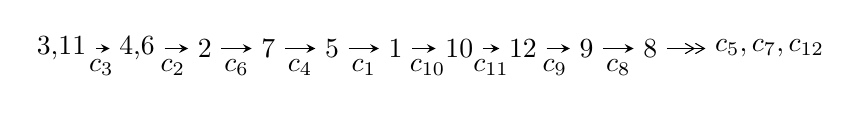
\begin{tikzpicture}[x=23pt, y=7pt]
	% node
	\node (A0) at (-1/8, 0) {3,11};
	\node (A1) at (17/16, 0) {4,6};
	\node (A2) at (17/8, 0) {2};
	\node (A3) at (25/8, 0) {7};
	\node (A4) at (33/8, 0) {5};
	\node (A5) at (41/8, 0) {1};
	\node (A6) at (49/8, 0) {10};
	\node (A7) at (57/8, 0) {12};
	\node (A8) at (65/8, 0) {9};
	\node (A9) at (73/8, 0) {8};
	\node (C1) at (1/2, -1) {$c_{3}$};
	\node (C2) at (13/8, -1) {$c_{2}$};
	\node (C3) at (21/8, -1) {$c_{6}$};
	\node (C4) at (29/8, -1) {$c_{4}$};
	\node (C5) at (37/8, -1) {$c_{1}$};
	\node (C6) at (45/8, -1) {$c_{10}$};
	\node (C7) at (53/8, -1) {$c_{11}$};
	\node (C8) at (61/8, -1) {$c_{9}$};
	\node (C9) at (69/8, -1) {$c_{8}$};
	\node (A10) at (11, 0) {$c_{5},c_{7},c_{12}$};

	% edge
	\draw[->,>=stealth]	
	(A0) edge (A1) (A1) edge (A2) (A2) edge (A3) (A3) edge (A4) (A4) edge (A5) (A5) edge (A6) (A6) edge (A7) (A7) edge (A8) (A8) edge (A9) ;
	\draw[->>,>={angle 60}]	
	(A9) edge (A10);
\end{tikzpicture} \\ 

\end{tabular} \\

\footnotetext{
The image of knot diagram is generated by the software ``\textbf{Draw programme}" developed by Andrew Bartholomew(\url{http://www.layer8.co.uk/maths/draw/index.htm\#Running-draw}), where we modified some parts for our purpose(\url{https://github.com/CATsTAILs/LinksPainter}).
}\phantom \\ \newline 
\centering \textbf{Ideals for irreducible components\footnotemark of $X_{\text{par}}$} 
 
\begin{align*}
I^u_{1}&=\langle 
2.55777\times10^{154} u^{87}+1.33040\times10^{154} u^{86}+\cdots+1.37278\times10^{154} b-6.08647\times10^{155},\\
\phantom{I^u_{1}}&\phantom{= \langle  }4.05262\times10^{155} u^{87}+2.19316\times10^{156} u^{86}+\cdots+3.02011\times10^{155} a+5.78829\times10^{157},\\
\phantom{I^u_{1}}&\phantom{= \langle  }u^{88}+2 u^{87}+\cdots+128 u+32\rangle \\
I^u_{2}&=\langle 
b,\;u^4+u^2+a+u,\;u^5- u^4+2 u^3- u^2+u-1\rangle \\
\\
I^v_{1}&=\langle 
a,\;-2 v^4+v^3+3 v^2+b-6 v+2,\;v^5- v^4- v^3+4 v^2-3 v+1\rangle \\
\end{align*}
\raggedright * 3 irreducible components of $\dim_{\mathbb{C}}=0$, with total 98 representations.\\
\footnotetext{All coefficients of polynomials are rational numbers. But the coefficients are sometimes approximated in decimal forms when there is not enough margin.}
\newpage
\renewcommand{\arraystretch}{1}
\centering \section*{I. $I^u_{1}= \langle 2.56\times10^{154} u^{87}+1.33\times10^{154} u^{86}+\cdots+1.37\times10^{154} b-6.09\times10^{155},\;4.05\times10^{155} u^{87}+2.19\times10^{156} u^{86}+\cdots+3.02\times10^{155} a+5.79\times10^{157},\;u^{88}+2 u^{87}+\cdots+128 u+32 \rangle$}
\flushleft \textbf{(i) Arc colorings}\\
\begin{tabular}{m{7pt} m{180pt} m{7pt} m{180pt} }
\flushright $a_{3}=$&$\begin{pmatrix}1\\0\end{pmatrix}$ \\
\flushright $a_{11}=$&$\begin{pmatrix}0\\u\end{pmatrix}$ \\
\flushright $a_{4}=$&$\begin{pmatrix}1\\u^2\end{pmatrix}$ \\
\flushright $a_{6}=$&$\begin{pmatrix}-1.34188 u^{87}-7.26185 u^{86}+\cdots-648.536 u-191.658\\-1.86321 u^{87}-0.969132 u^{86}+\cdots+62.2360 u+44.3369\end{pmatrix}$ \\
\flushright $a_{2}=$&$\begin{pmatrix}3.04936 u^{87}+5.94300 u^{86}+\cdots+329.238 u+75.2429\\-1.43574 u^{87}-2.17821 u^{86}+\cdots-23.2178 u+6.62152\end{pmatrix}$ \\
\flushright $a_{7}=$&$\begin{pmatrix}-4.53882 u^{87}-7.84119 u^{86}+\cdots-388.579 u-74.4637\\1.02928 u^{87}-2.25200 u^{86}+\cdots-369.905 u-130.560\end{pmatrix}$ \\
\flushright $a_{5}=$&$\begin{pmatrix}-0.0781229 u^{87}+1.92398 u^{86}+\cdots+185.114 u+62.4308\\-0.503789 u^{87}-3.88549 u^{86}+\cdots-424.089 u-133.649\end{pmatrix}$ \\
\flushright $a_{1}=$&$\begin{pmatrix}1.61362 u^{87}+3.76479 u^{86}+\cdots+306.020 u+81.8645\\-1.43574 u^{87}-2.17821 u^{86}+\cdots-23.2178 u+6.62152\end{pmatrix}$ \\
\flushright $a_{10}=$&$\begin{pmatrix}u\\u^3+u\end{pmatrix}$ \\
\flushright $a_{12}=$&$\begin{pmatrix}u^3\\u^5+u^3+u\end{pmatrix}$ \\
\flushright $a_{9}=$&$\begin{pmatrix}-1.55260 u^{87}-6.01547 u^{86}+\cdots-445.753 u-125.053\\1.59435 u^{87}+2.04652 u^{86}+\cdots+133.630 u+23.9040\end{pmatrix}$ \\
\flushright $a_{8}=$&$\begin{pmatrix}-3.04936 u^{87}-5.94300 u^{86}+\cdots-329.238 u-75.2429\\1.61315 u^{87}+1.25714 u^{86}+\cdots+54.4288 u+1.63829\end{pmatrix}$\\&\end{tabular}
\flushleft \textbf{(ii) Obstruction class $= -1$}\\~\\
\flushleft \textbf{(iii) Cusp Shapes $= 3.28609 u^{87}+5.01107 u^{86}+\cdots+173.927 u+44.2883$}\\~\\
\newpage\renewcommand{\arraystretch}{1}
\flushleft \textbf{(iv) u-Polynomials at the component}\newline \\
\begin{tabular}{m{50pt}|m{274pt}}
Crossings & \hspace{64pt}u-Polynomials at each crossing \\
\hline $$\begin{aligned}c_{1}\end{aligned}$$&$\begin{aligned}
&u^{88}+36 u^{87}+\cdots+3584 u+1024
\end{aligned}$\\
\hline $$\begin{aligned}c_{2},c_{6}\end{aligned}$$&$\begin{aligned}
&u^{88}-2 u^{87}+\cdots-128 u+32
\end{aligned}$\\
\hline $$\begin{aligned}c_{3},c_{10}\end{aligned}$$&$\begin{aligned}
&u^{88}+2 u^{87}+\cdots+128 u+32
\end{aligned}$\\
\hline $$\begin{aligned}c_{4},c_{5},c_{7}\end{aligned}$$&$\begin{aligned}
&u^{88}-7 u^{87}+\cdots+9 u-1
\end{aligned}$\\
\hline $$\begin{aligned}c_{8},c_{9},c_{12}\end{aligned}$$&$\begin{aligned}
&u^{88}+7 u^{87}+\cdots-9 u-1
\end{aligned}$\\
\hline $$\begin{aligned}c_{11}\end{aligned}$$&$\begin{aligned}
&u^{88}-36 u^{87}+\cdots-3584 u+1024
\end{aligned}$\\
\hline
\end{tabular}\\~\\
\newpage\renewcommand{\arraystretch}{1}
\flushleft \textbf{(v) Riley Polynomials at the component}\newline \\
\begin{tabular}{m{50pt}|m{274pt}}
Crossings & \hspace{64pt}Riley Polynomials at each crossing \\
\hline $$\begin{aligned}c_{1},c_{11}\end{aligned}$$&$\begin{aligned}
&y^{88}+24 y^{87}+\cdots-66715648 y+1048576
\end{aligned}$\\
\hline $$\begin{aligned}c_{2},c_{3},c_{6}\\c_{10}\end{aligned}$$&$\begin{aligned}
&y^{88}+36 y^{87}+\cdots+3584 y+1024
\end{aligned}$\\
\hline $$\begin{aligned}c_{4},c_{5},c_{7}\\c_{8},c_{9},c_{12}\end{aligned}$$&$\begin{aligned}
&y^{88}-77 y^{87}+\cdots-57 y+1
\end{aligned}$\\
\hline
\end{tabular}\\~\\
\newpage\flushleft \textbf{(vi) Complex Volumes and Cusp Shapes}
$$\begin{array}{c|c|c}  
\text{Solutions to }I^u_{1}& \I (\text{vol} + \sqrt{-1}CS) & \text{Cusp shape}\\
 \hline 
\begin{aligned}
u &= -0.395995 + 0.919848 I \\
a &= \phantom{-}2.65099 - 0.04295 I \\
b &= -0.586527 - 0.945687 I\end{aligned}
 & \phantom{-}2.26153 + 3.00983 I & \phantom{-0.000000 } 0 \\ \hline\begin{aligned}
u &= -0.395995 - 0.919848 I \\
a &= \phantom{-}2.65099 + 0.04295 I \\
b &= -0.586527 + 0.945687 I\end{aligned}
 & \phantom{-}2.26153 - 3.00983 I & \phantom{-0.000000 } 0 \\ \hline\begin{aligned}
u &= -0.404116 + 0.907512 I \\
a &= -0.395066 - 0.612626 I \\
b &= \phantom{-}0.361388 - 1.098660 I\end{aligned}
 & \phantom{-}2.25457 + 0.19023 I & \phantom{-0.000000 } 0 \\ \hline\begin{aligned}
u &= -0.404116 - 0.907512 I \\
a &= -0.395066 + 0.612626 I \\
b &= \phantom{-}0.361388 + 1.098660 I\end{aligned}
 & \phantom{-}2.25457 - 0.19023 I & \phantom{-0.000000 } 0 \\ \hline\begin{aligned}
u &= -0.886787 + 0.438676 I \\
a &= \phantom{-}0.282546 + 1.241530 I \\
b &= -0.415238 + 0.812588 I\end{aligned}
 & \phantom{-}0.69474 - 1.25403 I & \phantom{-0.000000 } 0 \\ \hline\begin{aligned}
u &= -0.886787 - 0.438676 I \\
a &= \phantom{-}0.282546 - 1.241530 I \\
b &= -0.415238 - 0.812588 I\end{aligned}
 & \phantom{-}0.69474 + 1.25403 I & \phantom{-0.000000 } 0 \\ \hline\begin{aligned}
u &= \phantom{-}0.812254 + 0.547196 I \\
a &= \phantom{-}0.436136 - 0.137542 I \\
b &= -0.616284 - 1.184160 I\end{aligned}
 & -6.80158 + 6.33791 I & \phantom{-0.000000 } 0 \\ \hline\begin{aligned}
u &= \phantom{-}0.812254 - 0.547196 I \\
a &= \phantom{-}0.436136 + 0.137542 I \\
b &= -0.616284 + 1.184160 I\end{aligned}
 & -6.80158 - 6.33791 I & \phantom{-0.000000 } 0 \\ \hline\begin{aligned}
u &= \phantom{-}0.474341 + 0.926493 I \\
a &= \phantom{-}1.015950 + 0.235751 I \\
b &= -1.123980 + 0.220654 I\end{aligned}
 & -0.22584 - 2.46461 I & \phantom{-0.000000 } 0 \\ \hline\begin{aligned}
u &= \phantom{-}0.474341 - 0.926493 I \\
a &= \phantom{-}1.015950 - 0.235751 I \\
b &= -1.123980 - 0.220654 I\end{aligned}
 & -0.22584 + 2.46461 I & \phantom{-0.000000 } 0\\
 \hline 
 \end{array}$$\newpage$$\begin{array}{c|c|c}  
\text{Solutions to }I^u_{1}& \I (\text{vol} + \sqrt{-1}CS) & \text{Cusp shape}\\
 \hline 
\begin{aligned}
u &= \phantom{-}0.625512 + 0.717766 I \\
a &= -0.175517 - 1.114280 I \\
b &= -0.159287 - 0.924776 I\end{aligned}
 & -2.96877 - 1.76029 I & \phantom{-0.000000 } 0 \\ \hline\begin{aligned}
u &= \phantom{-}0.625512 - 0.717766 I \\
a &= -0.175517 + 1.114280 I \\
b &= -0.159287 + 0.924776 I\end{aligned}
 & -2.96877 + 1.76029 I & \phantom{-0.000000 } 0 \\ \hline\begin{aligned}
u &= \phantom{-}0.995359 + 0.339245 I \\
a &= -0.580860 - 0.374909 I \\
b &= \phantom{-}0.678568 - 0.640826 I\end{aligned}
 & \phantom{-}4.14234 + 0.58263 I & \phantom{-0.000000 } 0 \\ \hline\begin{aligned}
u &= \phantom{-}0.995359 - 0.339245 I \\
a &= -0.580860 + 0.374909 I \\
b &= \phantom{-}0.678568 + 0.640826 I\end{aligned}
 & \phantom{-}4.14234 - 0.58263 I & \phantom{-0.000000 } 0 \\ \hline\begin{aligned}
u &= \phantom{-}0.159287 + 0.924776 I \\
a &= \phantom{-}1.36498 + 1.59127 I \\
b &= -0.625512 - 0.717766 I\end{aligned}
 & \phantom{-}2.96877 + 1.76029 I & \phantom{-0.000000 } 0 \\ \hline\begin{aligned}
u &= \phantom{-}0.159287 - 0.924776 I \\
a &= \phantom{-}1.36498 - 1.59127 I \\
b &= -0.625512 + 0.717766 I\end{aligned}
 & \phantom{-}2.96877 - 1.76029 I & \phantom{-0.000000 } 0 \\ \hline\begin{aligned}
u &= -0.678568 + 0.640826 I \\
a &= \phantom{-}1.063540 - 0.436699 I \\
b &= -0.995359 - 0.339245 I\end{aligned}
 & -4.14234 - 0.58263 I & \phantom{-0.000000 } 0 \\ \hline\begin{aligned}
u &= -0.678568 - 0.640826 I \\
a &= \phantom{-}1.063540 + 0.436699 I \\
b &= -0.995359 + 0.339245 I\end{aligned}
 & -4.14234 + 0.58263 I & \phantom{-0.000000 } 0 \\ \hline\begin{aligned}
u &= \phantom{-}0.073976 + 1.077970 I \\
a &= -1.08508 - 1.73052 I \\
b &= \phantom{-}0.521667 + 0.977886 I\end{aligned}
 & -1.30307 + 4.99629 I & \phantom{-0.000000 } 0 \\ \hline\begin{aligned}
u &= \phantom{-}0.073976 - 1.077970 I \\
a &= -1.08508 + 1.73052 I \\
b &= \phantom{-}0.521667 - 0.977886 I\end{aligned}
 & -1.30307 - 4.99629 I & \phantom{-0.000000 } 0\\
 \hline 
 \end{array}$$\newpage$$\begin{array}{c|c|c}  
\text{Solutions to }I^u_{1}& \I (\text{vol} + \sqrt{-1}CS) & \text{Cusp shape}\\
 \hline 
\begin{aligned}
u &= \phantom{-}0.958984 + 0.503942 I \\
a &= \phantom{-}0.926029 + 0.597774 I \\
b &= -0.958984 + 0.503942 I\end{aligned}
 & \phantom{-0.000000 -}3.72374 I & \phantom{-0.000000 } 0 \\ \hline\begin{aligned}
u &= \phantom{-}0.958984 - 0.503942 I \\
a &= \phantom{-}0.926029 - 0.597774 I \\
b &= -0.958984 - 0.503942 I\end{aligned}
 & \phantom{-0.000000 } -3.72374 I & \phantom{-0.000000 } 0 \\ \hline\begin{aligned}
u &= \phantom{-}0.415238 + 0.812588 I \\
a &= -1.44367 - 1.70184 I \\
b &= \phantom{-}0.886787 + 0.438676 I\end{aligned}
 & -0.69474 - 1.25403 I & \phantom{-0.000000 } 0 \\ \hline\begin{aligned}
u &= \phantom{-}0.415238 - 0.812588 I \\
a &= -1.44367 + 1.70184 I \\
b &= \phantom{-}0.886787 - 0.438676 I\end{aligned}
 & -0.69474 + 1.25403 I & \phantom{-0.000000 } 0 \\ \hline\begin{aligned}
u &= \phantom{-}0.702985 + 0.565831 I \\
a &= -0.460163 + 0.540285 I \\
b &= \phantom{-}0.495675 + 0.994508 I\end{aligned}
 & -1.40784 + 2.54267 I & -3.45686 - 3.29238 I \\ \hline\begin{aligned}
u &= \phantom{-}0.702985 - 0.565831 I \\
a &= -0.460163 - 0.540285 I \\
b &= \phantom{-}0.495675 - 0.994508 I\end{aligned}
 & -1.40784 - 2.54267 I & -3.45686 + 3.29238 I \\ \hline\begin{aligned}
u &= -0.521667 + 0.977886 I \\
a &= -0.200965 + 0.894250 I \\
b &= -0.073976 + 1.077970 I\end{aligned}
 & \phantom{-}1.30307 + 4.99629 I & \phantom{-0.000000 } 0 \\ \hline\begin{aligned}
u &= -0.521667 - 0.977886 I \\
a &= -0.200965 - 0.894250 I \\
b &= -0.073976 - 1.077970 I\end{aligned}
 & \phantom{-}1.30307 - 4.99629 I & \phantom{-0.000000 } 0 \\ \hline\begin{aligned}
u &= -0.495675 + 0.994508 I \\
a &= \phantom{-}0.546599 - 1.120560 I \\
b &= -0.702985 + 0.565831 I\end{aligned}
 & \phantom{-}1.40784 + 2.54267 I & \phantom{-0.000000 } 0 \\ \hline\begin{aligned}
u &= -0.495675 - 0.994508 I \\
a &= \phantom{-}0.546599 + 1.120560 I \\
b &= -0.702985 - 0.565831 I\end{aligned}
 & \phantom{-}1.40784 - 2.54267 I & \phantom{-0.000000 } 0\\
 \hline 
 \end{array}$$\newpage$$\begin{array}{c|c|c}  
\text{Solutions to }I^u_{1}& \I (\text{vol} + \sqrt{-1}CS) & \text{Cusp shape}\\
 \hline 
\begin{aligned}
u &= -0.798601 + 0.772998 I \\
a &= \phantom{-}1.096920 - 0.166790 I \\
b &= \phantom{-}0.033875 - 1.258740 I\end{aligned}
 & -6.87603 - 1.37349 I & \phantom{-0.000000 } 0 \\ \hline\begin{aligned}
u &= -0.798601 - 0.772998 I \\
a &= \phantom{-}1.096920 + 0.166790 I \\
b &= \phantom{-}0.033875 + 1.258740 I\end{aligned}
 & -6.87603 + 1.37349 I & \phantom{-0.000000 } 0 \\ \hline\begin{aligned}
u &= \phantom{-}0.586527 + 0.945687 I \\
a &= -1.79270 - 1.01470 I \\
b &= \phantom{-}0.395995 - 0.919848 I\end{aligned}
 & -2.26153 - 3.00983 I & \phantom{-0.000000 } 0 \\ \hline\begin{aligned}
u &= \phantom{-}0.586527 - 0.945687 I \\
a &= -1.79270 + 1.01470 I \\
b &= \phantom{-}0.395995 + 0.919848 I\end{aligned}
 & -2.26153 + 3.00983 I & \phantom{-0.000000 } 0 \\ \hline\begin{aligned}
u &= -0.471722 + 1.010740 I \\
a &= -2.48364 - 0.23893 I \\
b &= \phantom{-}0.651889 + 1.129260 I\end{aligned}
 & -2.77315 + 6.92377 I & \phantom{-0.000000 } 0 \\ \hline\begin{aligned}
u &= -0.471722 - 1.010740 I \\
a &= -2.48364 + 0.23893 I \\
b &= \phantom{-}0.651889 - 1.129260 I\end{aligned}
 & -2.77315 - 6.92377 I & \phantom{-0.000000 } 0 \\ \hline\begin{aligned}
u &= -1.021560 + 0.502568 I \\
a &= -0.452502 - 0.480269 I \\
b &= \phantom{-}0.617119 - 0.992602 I\end{aligned}
 & \phantom{-}3.07312 - 5.61606 I & \phantom{-0.000000 } 0 \\ \hline\begin{aligned}
u &= -1.021560 - 0.502568 I \\
a &= -0.452502 + 0.480269 I \\
b &= \phantom{-}0.617119 + 0.992602 I\end{aligned}
 & \phantom{-}3.07312 + 5.61606 I & \phantom{-0.000000 } 0 \\ \hline\begin{aligned}
u &= \phantom{-}1.123980 + 0.220654 I \\
a &= \phantom{-}0.425729 + 0.019981 I \\
b &= -0.474341 + 0.926493 I\end{aligned}
 & \phantom{-}0.22584 - 2.46461 I & \phantom{-0.000000 } 0 \\ \hline\begin{aligned}
u &= \phantom{-}1.123980 - 0.220654 I \\
a &= \phantom{-}0.425729 - 0.019981 I \\
b &= -0.474341 - 0.926493 I\end{aligned}
 & \phantom{-}0.22584 + 2.46461 I & \phantom{-0.000000 } 0\\
 \hline 
 \end{array}$$\newpage$$\begin{array}{c|c|c}  
\text{Solutions to }I^u_{1}& \I (\text{vol} + \sqrt{-1}CS) & \text{Cusp shape}\\
 \hline 
\begin{aligned}
u &= \phantom{-}0.769853 + 0.852318 I \\
a &= \phantom{-}0.864593 + 0.257379 I \\
b &= -0.066555 + 1.321620 I\end{aligned}
 & -10.45800 - 2.88090 I & \phantom{-0.000000 } 0 \\ \hline\begin{aligned}
u &= \phantom{-}0.769853 - 0.852318 I \\
a &= \phantom{-}0.864593 - 0.257379 I \\
b &= -0.066555 - 1.321620 I\end{aligned}
 & -10.45800 + 2.88090 I & \phantom{-0.000000 } 0 \\ \hline\begin{aligned}
u &= -0.361388 + 1.098660 I \\
a &= -0.11965 + 1.46530 I \\
b &= \phantom{-}0.404116 - 0.907512 I\end{aligned}
 & -2.25457 - 0.19023 I & \phantom{-0.000000 } 0 \\ \hline\begin{aligned}
u &= -0.361388 - 1.098660 I \\
a &= -0.11965 - 1.46530 I \\
b &= \phantom{-}0.404116 + 0.907512 I\end{aligned}
 & -2.25457 + 0.19023 I & \phantom{-0.000000 } 0 \\ \hline\begin{aligned}
u &= -0.358618 + 0.763180 I \\
a &= \phantom{-}0.471283 + 0.174177 I \\
b &= -0.537085 + 1.290420 I\end{aligned}
 & -3.83566 - 3.43814 I & \phantom{-}0.61318 - 1.44912 I \\ \hline\begin{aligned}
u &= -0.358618 - 0.763180 I \\
a &= \phantom{-}0.471283 - 0.174177 I \\
b &= -0.537085 - 1.290420 I\end{aligned}
 & -3.83566 + 3.43814 I & \phantom{-}0.61318 + 1.44912 I \\ \hline\begin{aligned}
u &= -0.684043 + 0.947304 I \\
a &= \phantom{-}0.721420 - 0.287781 I \\
b &= -0.157119 - 1.376880 I\end{aligned}
 & -6.29574 + 6.95849 I & \phantom{-0.000000 } 0 \\ \hline\begin{aligned}
u &= -0.684043 - 0.947304 I \\
a &= \phantom{-}0.721420 + 0.287781 I \\
b &= -0.157119 + 1.376880 I\end{aligned}
 & -6.29574 - 6.95849 I & \phantom{-0.000000 } 0 \\ \hline\begin{aligned}
u &= -0.617119 + 0.992602 I \\
a &= -0.89496 + 1.13273 I \\
b &= \phantom{-}1.021560 - 0.502568 I\end{aligned}
 & -3.07312 + 5.61606 I & \phantom{-0.000000 } 0 \\ \hline\begin{aligned}
u &= -0.617119 - 0.992602 I \\
a &= -0.89496 - 1.13273 I \\
b &= \phantom{-}1.021560 + 0.502568 I\end{aligned}
 & -3.07312 - 5.61606 I & \phantom{-0.000000 } 0\\
 \hline 
 \end{array}$$\newpage$$\begin{array}{c|c|c}  
\text{Solutions to }I^u_{1}& \I (\text{vol} + \sqrt{-1}CS) & \text{Cusp shape}\\
 \hline 
\begin{aligned}
u &= \phantom{-}0.443550 + 1.114320 I \\
a &= -0.636408 - 0.138775 I \\
b &= \phantom{-}0.637561 - 0.134384 I\end{aligned}
 & \phantom{-}5.24580 - 3.85196 I & \phantom{-0.000000 } 0 \\ \hline\begin{aligned}
u &= \phantom{-}0.443550 - 1.114320 I \\
a &= -0.636408 + 0.138775 I \\
b &= \phantom{-}0.637561 + 0.134384 I\end{aligned}
 & \phantom{-}5.24580 + 3.85196 I & \phantom{-0.000000 } 0 \\ \hline\begin{aligned}
u &= \phantom{-}0.613830 + 1.034560 I \\
a &= \phantom{-}2.09577 + 0.54409 I \\
b &= -0.613830 + 1.034560 I\end{aligned}
 & \phantom{-0.000000 } -7.63074 I & \phantom{-0.000000 } 0 \\ \hline\begin{aligned}
u &= \phantom{-}0.613830 - 1.034560 I \\
a &= \phantom{-}2.09577 - 0.54409 I \\
b &= -0.613830 - 1.034560 I\end{aligned}
 & \phantom{-0.000000 -}7.63074 I & \phantom{-0.000000 } 0 \\ \hline\begin{aligned}
u &= -0.365401 + 0.697232 I \\
a &= -0.790767 + 0.184744 I \\
b &= \phantom{-}0.430621 + 0.240473 I\end{aligned}
 & \phantom{-}0.192499 + 1.200880 I & \phantom{-}3.44276 - 4.83413 I \\ \hline\begin{aligned}
u &= -0.365401 - 0.697232 I \\
a &= -0.790767 - 0.184744 I \\
b &= \phantom{-}0.430621 - 0.240473 I\end{aligned}
 & \phantom{-}0.192499 - 1.200880 I & \phantom{-}3.44276 + 4.83413 I \\ \hline\begin{aligned}
u &= -1.078720 + 0.561603 I \\
a &= \phantom{-}0.410171 + 0.130932 I \\
b &= -0.687566 + 1.140520 I\end{aligned}
 & -1.99246 - 9.73563 I & \phantom{-0.000000 } 0 \\ \hline\begin{aligned}
u &= -1.078720 - 0.561603 I \\
a &= \phantom{-}0.410171 - 0.130932 I \\
b &= -0.687566 - 1.140520 I\end{aligned}
 & -1.99246 + 9.73563 I & \phantom{-0.000000 } 0 \\ \hline\begin{aligned}
u &= -0.033875 + 1.258740 I \\
a &= -1.59344 + 0.20088 I \\
b &= \phantom{-}0.798601 - 0.772998 I\end{aligned}
 & \phantom{-}6.87603 + 1.37349 I & \phantom{-0.000000 } 0 \\ \hline\begin{aligned}
u &= -0.033875 - 1.258740 I \\
a &= -1.59344 - 0.20088 I \\
b &= \phantom{-}0.798601 + 0.772998 I\end{aligned}
 & \phantom{-}6.87603 - 1.37349 I & \phantom{-0.000000 } 0\\
 \hline 
 \end{array}$$\newpage$$\begin{array}{c|c|c}  
\text{Solutions to }I^u_{1}& \I (\text{vol} + \sqrt{-1}CS) & \text{Cusp shape}\\
 \hline 
\begin{aligned}
u &= \phantom{-}0.655409 + 1.077200 I \\
a &= -2.11903 - 0.25132 I \\
b &= \phantom{-}0.703968 - 1.167180 I\end{aligned}
 & -5.18587 - 11.86060 I & \phantom{-0.000000 } 0 \\ \hline\begin{aligned}
u &= \phantom{-}0.655409 - 1.077200 I \\
a &= -2.11903 + 0.25132 I \\
b &= \phantom{-}0.703968 + 1.167180 I\end{aligned}
 & -5.18587 + 11.86060 I & \phantom{-0.000000 } 0 \\ \hline\begin{aligned}
u &= -0.119816 + 0.724230 I \\
a &= -3.31363 + 0.21378 I \\
b &= \phantom{-}0.496811 + 0.533389 I\end{aligned}
 & -0.110831 - 0.799402 I & \phantom{-}3.78510 - 2.23405 I \\ \hline\begin{aligned}
u &= -0.119816 - 0.724230 I \\
a &= -3.31363 - 0.21378 I \\
b &= \phantom{-}0.496811 - 0.533389 I\end{aligned}
 & -0.110831 + 0.799402 I & \phantom{-}3.78510 + 2.23405 I \\ \hline\begin{aligned}
u &= -0.496811 + 0.533389 I \\
a &= -2.32822 + 1.78680 I \\
b &= \phantom{-}0.119816 + 0.724230 I\end{aligned}
 & \phantom{-}0.110831 - 0.799402 I & -3.78510 - 2.23405 I \\ \hline\begin{aligned}
u &= -0.496811 - 0.533389 I \\
a &= -2.32822 - 1.78680 I \\
b &= \phantom{-}0.119816 - 0.724230 I\end{aligned}
 & \phantom{-}0.110831 + 0.799402 I & -3.78510 + 2.23405 I \\ \hline\begin{aligned}
u &= -0.651889 + 1.129260 I \\
a &= -1.52240 + 0.84713 I \\
b &= \phantom{-}0.471722 + 1.010740 I\end{aligned}
 & \phantom{-}2.77315 + 6.92377 I & \phantom{-0.000000 } 0 \\ \hline\begin{aligned}
u &= -0.651889 - 1.129260 I \\
a &= -1.52240 - 0.84713 I \\
b &= \phantom{-}0.471722 - 1.010740 I\end{aligned}
 & \phantom{-}2.77315 - 6.92377 I & \phantom{-0.000000 } 0 \\ \hline\begin{aligned}
u &= \phantom{-}0.066555 + 1.321620 I \\
a &= \phantom{-}1.45861 - 0.47999 I \\
b &= -0.769853 + 0.852318 I\end{aligned}
 & \phantom{-}10.45800 - 2.88090 I & \phantom{-0.000000 } 0 \\ \hline\begin{aligned}
u &= \phantom{-}0.066555 - 1.321620 I \\
a &= \phantom{-}1.45861 + 0.47999 I \\
b &= -0.769853 - 0.852318 I\end{aligned}
 & \phantom{-}10.45800 + 2.88090 I & \phantom{-0.000000 } 0\\
 \hline 
 \end{array}$$\newpage$$\begin{array}{c|c|c}  
\text{Solutions to }I^u_{1}& \I (\text{vol} + \sqrt{-1}CS) & \text{Cusp shape}\\
 \hline 
\begin{aligned}
u &= \phantom{-}0.687566 + 1.140520 I \\
a &= -0.821367 - 0.858877 I \\
b &= \phantom{-}1.078720 + 0.561603 I\end{aligned}
 & \phantom{-}1.99246 - 9.73563 I & \phantom{-0.000000 } 0 \\ \hline\begin{aligned}
u &= \phantom{-}0.687566 - 1.140520 I \\
a &= -0.821367 + 0.858877 I \\
b &= \phantom{-}1.078720 - 0.561603 I\end{aligned}
 & \phantom{-}1.99246 + 9.73563 I & \phantom{-0.000000 } 0 \\ \hline\begin{aligned}
u &= \phantom{-}0.616284 + 1.184160 I \\
a &= \phantom{-}0.579368 + 0.788710 I \\
b &= -0.812254 - 0.547196 I\end{aligned}
 & \phantom{-}6.80158 - 6.33791 I & \phantom{-0.000000 } 0 \\ \hline\begin{aligned}
u &= \phantom{-}0.616284 - 1.184160 I \\
a &= \phantom{-}0.579368 - 0.788710 I \\
b &= -0.812254 + 0.547196 I\end{aligned}
 & \phantom{-}6.80158 + 6.33791 I & \phantom{-0.000000 } 0 \\ \hline\begin{aligned}
u &= -0.637561 + 0.134384 I \\
a &= \phantom{-}0.495827 - 0.083510 I \\
b &= -0.443550 - 1.114320 I\end{aligned}
 & -5.24580 + 3.85196 I & -8.95635 - 3.01207 I \\ \hline\begin{aligned}
u &= -0.637561 - 0.134384 I \\
a &= \phantom{-}0.495827 + 0.083510 I \\
b &= -0.443550 + 1.114320 I\end{aligned}
 & -5.24580 - 3.85196 I & -8.95635 + 3.01207 I \\ \hline\begin{aligned}
u &= \phantom{-}0.645090\phantom{ +0.000000I} \\
a &= -0.735762\phantom{ +0.000000I} \\
b &= -0.330483\phantom{ +0.000000I}\end{aligned}
 & \phantom{-}2.22439\phantom{ +0.000000I} & \phantom{-}4.34230\phantom{ +0.000000I} \\ \hline\begin{aligned}
u &= -0.703968 + 1.167180 I \\
a &= \phantom{-}1.76924 - 0.55256 I \\
b &= -0.655409 - 1.077200 I\end{aligned}
 & \phantom{-}5.18587 + 11.86060 I & \phantom{-0.000000 } 0 \\ \hline\begin{aligned}
u &= -0.703968 - 1.167180 I \\
a &= \phantom{-}1.76924 + 0.55256 I \\
b &= -0.655409 + 1.077200 I\end{aligned}
 & \phantom{-}5.18587 - 11.86060 I & \phantom{-0.000000 } 0 \\ \hline\begin{aligned}
u &= \phantom{-}0.157119 + 1.376880 I \\
a &= -1.29707 + 0.71694 I \\
b &= \phantom{-}0.684043 - 0.947304 I\end{aligned}
 & \phantom{-}6.29574 - 6.95849 I & \phantom{-0.000000 } 0\\
 \hline 
 \end{array}$$\newpage$$\begin{array}{c|c|c}  
\text{Solutions to }I^u_{1}& \I (\text{vol} + \sqrt{-1}CS) & \text{Cusp shape}\\
 \hline 
\begin{aligned}
u &= \phantom{-}0.157119 - 1.376880 I \\
a &= -1.29707 - 0.71694 I \\
b &= \phantom{-}0.684043 + 0.947304 I\end{aligned}
 & \phantom{-}6.29574 + 6.95849 I & \phantom{-0.000000 } 0 \\ \hline\begin{aligned}
u &= -0.748964 + 1.177590 I \\
a &= -1.81834 + 0.32952 I \\
b &= \phantom{-}0.748964 + 1.177590 I\end{aligned}
 & \phantom{-0.000000 -}16.3231 I & \phantom{-0.000000 } 0 \\ \hline\begin{aligned}
u &= -0.748964 - 1.177590 I \\
a &= -1.81834 - 0.32952 I \\
b &= \phantom{-}0.748964 - 1.177590 I\end{aligned}
 & \phantom{-0.000000 } -16.3231 I & \phantom{-0.000000 } 0 \\ \hline\begin{aligned}
u &= \phantom{-}0.537085 + 1.290420 I \\
a &= -0.079296 - 0.880909 I \\
b &= \phantom{-}0.358618 + 0.763180 I\end{aligned}
 & \phantom{-}3.83566 - 3.43814 I & \phantom{-0.000000 } 0 \\ \hline\begin{aligned}
u &= \phantom{-}0.537085 - 1.290420 I \\
a &= -0.079296 + 0.880909 I \\
b &= \phantom{-}0.358618 - 0.763180 I\end{aligned}
 & \phantom{-}3.83566 + 3.43814 I & \phantom{-0.000000 } 0 \\ \hline\begin{aligned}
u &= -0.430621 + 0.240473 I \\
a &= -0.693685 + 0.556563 I \\
b &= \phantom{-}0.365401 + 0.697232 I\end{aligned}
 & -0.192499 + 1.200880 I & -3.44276 - 4.83413 I \\ \hline\begin{aligned}
u &= -0.430621 - 0.240473 I \\
a &= -0.693685 - 0.556563 I \\
b &= \phantom{-}0.365401 - 0.697232 I\end{aligned}
 & -0.192499 - 1.200880 I & -3.44276 + 4.83413 I \\ \hline\begin{aligned}
u &= \phantom{-}0.330483\phantom{ +0.000000I} \\
a &= \phantom{-}2.08127\phantom{ +0.000000I} \\
b &= -0.645090\phantom{ +0.000000I}\end{aligned}
 & -2.22439\phantom{ +0.000000I} & -4.34230\phantom{ +0.000000I}\\
 \hline 
 \end{array}$$\newpage\newpage\renewcommand{\arraystretch}{1}
\centering \section*{II. $I^u_{2}= \langle b,\;u^4+u^2+a+u,\;u^5- u^4+2 u^3- u^2+u-1 \rangle$}
\flushleft \textbf{(i) Arc colorings}\\
\begin{tabular}{m{7pt} m{180pt} m{7pt} m{180pt} }
\flushright $a_{3}=$&$\begin{pmatrix}1\\0\end{pmatrix}$ \\
\flushright $a_{11}=$&$\begin{pmatrix}0\\u\end{pmatrix}$ \\
\flushright $a_{4}=$&$\begin{pmatrix}1\\u^2\end{pmatrix}$ \\
\flushright $a_{6}=$&$\begin{pmatrix}- u^4- u^2- u\\0\end{pmatrix}$ \\
\flushright $a_{2}=$&$\begin{pmatrix}1\\0\end{pmatrix}$ \\
\flushright $a_{7}=$&$\begin{pmatrix}- u^4- u^2- u\\0\end{pmatrix}$ \\
\flushright $a_{5}=$&$\begin{pmatrix}- u^4- u^2- u+1\\u^2\end{pmatrix}$ \\
\flushright $a_{1}=$&$\begin{pmatrix}1\\0\end{pmatrix}$ \\
\flushright $a_{10}=$&$\begin{pmatrix}u\\u^3+u\end{pmatrix}$ \\
\flushright $a_{12}=$&$\begin{pmatrix}u^3\\u^4- u^3+u^2+1\end{pmatrix}$ \\
\flushright $a_{9}=$&$\begin{pmatrix}- u^3\\u^3+u\end{pmatrix}$ \\
\flushright $a_{8}=$&$\begin{pmatrix}-1\\- u^2\end{pmatrix}$\\&\end{tabular}
\flushleft \textbf{(ii) Obstruction class $= 1$}\\~\\
\flushleft \textbf{(iii) Cusp Shapes $= -2 u^4-3 u^3+u^2-3 u$}\\~\\
\newpage\renewcommand{\arraystretch}{1}
\flushleft \textbf{(iv) u-Polynomials at the component}\newline \\
\begin{tabular}{m{50pt}|m{274pt}}
Crossings & \hspace{64pt}u-Polynomials at each crossing \\
\hline $$\begin{aligned}c_{1},c_{2},c_{6}\end{aligned}$$&$\begin{aligned}
&u^5
\end{aligned}$\\
\hline $$\begin{aligned}c_{3}\end{aligned}$$&$\begin{aligned}
&u^5- u^4+2 u^3- u^2+u-1
\end{aligned}$\\
\hline $$\begin{aligned}c_{4},c_{5}\end{aligned}$$&$\begin{aligned}
&(u-1)^5
\end{aligned}$\\
\hline $$\begin{aligned}c_{7}\end{aligned}$$&$\begin{aligned}
&(u+1)^5
\end{aligned}$\\
\hline $$\begin{aligned}c_{8},c_{9}\end{aligned}$$&$\begin{aligned}
&u^5- u^4-2 u^3+u^2+u+1
\end{aligned}$\\
\hline $$\begin{aligned}c_{10}\end{aligned}$$&$\begin{aligned}
&u^5+u^4+2 u^3+u^2+u+1
\end{aligned}$\\
\hline $$\begin{aligned}c_{11}\end{aligned}$$&$\begin{aligned}
&u^5-3 u^4+4 u^3- u^2- u+1
\end{aligned}$\\
\hline $$\begin{aligned}c_{12}\end{aligned}$$&$\begin{aligned}
&u^5+u^4-2 u^3- u^2+u-1
\end{aligned}$\\
\hline
\end{tabular}\\~\\
\newpage\renewcommand{\arraystretch}{1}
\flushleft \textbf{(v) Riley Polynomials at the component}\newline \\
\begin{tabular}{m{50pt}|m{274pt}}
Crossings & \hspace{64pt}Riley Polynomials at each crossing \\
\hline $$\begin{aligned}c_{1},c_{2},c_{6}\end{aligned}$$&$\begin{aligned}
&y^5
\end{aligned}$\\
\hline $$\begin{aligned}c_{3},c_{10}\end{aligned}$$&$\begin{aligned}
&y^5+3 y^4+4 y^3+y^2- y-1
\end{aligned}$\\
\hline $$\begin{aligned}c_{4},c_{5},c_{7}\end{aligned}$$&$\begin{aligned}
&(y-1)^5
\end{aligned}$\\
\hline $$\begin{aligned}c_{8},c_{9},c_{12}\end{aligned}$$&$\begin{aligned}
&y^5-5 y^4+8 y^3-3 y^2- y-1
\end{aligned}$\\
\hline $$\begin{aligned}c_{11}\end{aligned}$$&$\begin{aligned}
&y^5- y^4+8 y^3-3 y^2+3 y-1
\end{aligned}$\\
\hline
\end{tabular}\\~\\
\newpage\flushleft \textbf{(vi) Complex Volumes and Cusp Shapes}
$$\begin{array}{c|c|c}  
\text{Solutions to }I^u_{2}& \I (\text{vol} + \sqrt{-1}CS) & \text{Cusp shape}\\
 \hline 
\begin{aligned}
u &= -0.339110 + 0.822375 I \\
a &= \phantom{-}0.896438 - 0.890762 I \\
b &= \phantom{-0.000000 } 0\end{aligned}
 & -1.31583 + 1.53058 I & -1.49901 - 3.45976 I \\ \hline\begin{aligned}
u &= -0.339110 - 0.822375 I \\
a &= \phantom{-}0.896438 + 0.890762 I \\
b &= \phantom{-0.000000 } 0\end{aligned}
 & -1.31583 - 1.53058 I & -1.49901 + 3.45976 I \\ \hline\begin{aligned}
u &= \phantom{-}0.766826\phantom{ +0.000000I} \\
a &= -1.70062\phantom{ +0.000000I} \\
b &= \phantom{-0.000000 } 0\end{aligned}
 & \phantom{-}0.756147\phantom{ +0.000000I} & -3.75670\phantom{ +0.000000I} \\ \hline\begin{aligned}
u &= \phantom{-}0.455697 + 1.200150 I \\
a &= \phantom{-}0.453870 + 0.402731 I \\
b &= \phantom{-0.000000 } 0\end{aligned}
 & \phantom{-}4.22763 - 4.40083 I & \phantom{-}2.37737 + 5.82971 I \\ \hline\begin{aligned}
u &= \phantom{-}0.455697 - 1.200150 I \\
a &= \phantom{-}0.453870 - 0.402731 I \\
b &= \phantom{-0.000000 } 0\end{aligned}
 & \phantom{-}4.22763 + 4.40083 I & \phantom{-}2.37737 - 5.82971 I\\
 \hline 
 \end{array}$$\newpage\newpage\renewcommand{\arraystretch}{1}
\centering \section*{III. $I^v_{1}= \langle a,\;-2 v^4+v^3+3 v^2+b-6 v+2,\;v^5- v^4- v^3+4 v^2-3 v+1 \rangle$}
\flushleft \textbf{(i) Arc colorings}\\
\begin{tabular}{m{7pt} m{180pt} m{7pt} m{180pt} }
\flushright $a_{3}=$&$\begin{pmatrix}1\\0\end{pmatrix}$ \\
\flushright $a_{11}=$&$\begin{pmatrix}v\\0\end{pmatrix}$ \\
\flushright $a_{4}=$&$\begin{pmatrix}1\\0\end{pmatrix}$ \\
\flushright $a_{6}=$&$\begin{pmatrix}0\\2 v^4- v^3-3 v^2+6 v-2\end{pmatrix}$ \\
\flushright $a_{2}=$&$\begin{pmatrix}1\\v^4- v^3- v^2+4 v-3\end{pmatrix}$ \\
\flushright $a_{7}=$&$\begin{pmatrix}2 v^4- v^3-3 v^2+6 v-2\\- v^3+v-2\end{pmatrix}$ \\
\flushright $a_{5}=$&$\begin{pmatrix}-2 v^4+v^3+3 v^2-7 v+3\\v^3-2 v+3\end{pmatrix}$ \\
\flushright $a_{1}=$&$\begin{pmatrix}v^4- v^3- v^2+4 v-2\\v^4- v^3- v^2+4 v-3\end{pmatrix}$ \\
\flushright $a_{10}=$&$\begin{pmatrix}v\\0\end{pmatrix}$ \\
\flushright $a_{12}=$&$\begin{pmatrix}v\\0\end{pmatrix}$ \\
\flushright $a_{9}=$&$\begin{pmatrix}- v^4+v^3+v^2-3 v+2\\- v^4+v^3+v^2-4 v+3\end{pmatrix}$ \\
\flushright $a_{8}=$&$\begin{pmatrix}- v^4+v^3+v^2-4 v+2\\- v^4+v^3+v^2-4 v+3\end{pmatrix}$\\&\end{tabular}
\flushleft \textbf{(ii) Obstruction class $= 1$}\\~\\
\flushleft \textbf{(iii) Cusp Shapes $= -7 v^4+2 v^3+9 v^2-23 v+7$}\\~\\
\newpage\renewcommand{\arraystretch}{1}
\flushleft \textbf{(iv) u-Polynomials at the component}\newline \\
\begin{tabular}{m{50pt}|m{274pt}}
Crossings & \hspace{64pt}u-Polynomials at each crossing \\
\hline $$\begin{aligned}c_{1}\end{aligned}$$&$\begin{aligned}
&u^5-3 u^4+4 u^3- u^2- u+1
\end{aligned}$\\
\hline $$\begin{aligned}c_{2}\end{aligned}$$&$\begin{aligned}
&u^5- u^4+2 u^3- u^2+u-1
\end{aligned}$\\
\hline $$\begin{aligned}c_{3},c_{10},c_{11}\end{aligned}$$&$\begin{aligned}
&u^5
\end{aligned}$\\
\hline $$\begin{aligned}c_{4},c_{5}\end{aligned}$$&$\begin{aligned}
&u^5+u^4-2 u^3- u^2+u-1
\end{aligned}$\\
\hline $$\begin{aligned}c_{6}\end{aligned}$$&$\begin{aligned}
&u^5+u^4+2 u^3+u^2+u+1
\end{aligned}$\\
\hline $$\begin{aligned}c_{7}\end{aligned}$$&$\begin{aligned}
&u^5- u^4-2 u^3+u^2+u+1
\end{aligned}$\\
\hline $$\begin{aligned}c_{8},c_{9}\end{aligned}$$&$\begin{aligned}
&(u+1)^5
\end{aligned}$\\
\hline $$\begin{aligned}c_{12}\end{aligned}$$&$\begin{aligned}
&(u-1)^5
\end{aligned}$\\
\hline
\end{tabular}\\~\\
\newpage\renewcommand{\arraystretch}{1}
\flushleft \textbf{(v) Riley Polynomials at the component}\newline \\
\begin{tabular}{m{50pt}|m{274pt}}
Crossings & \hspace{64pt}Riley Polynomials at each crossing \\
\hline $$\begin{aligned}c_{1}\end{aligned}$$&$\begin{aligned}
&y^5- y^4+8 y^3-3 y^2+3 y-1
\end{aligned}$\\
\hline $$\begin{aligned}c_{2},c_{6}\end{aligned}$$&$\begin{aligned}
&y^5+3 y^4+4 y^3+y^2- y-1
\end{aligned}$\\
\hline $$\begin{aligned}c_{3},c_{10},c_{11}\end{aligned}$$&$\begin{aligned}
&y^5
\end{aligned}$\\
\hline $$\begin{aligned}c_{4},c_{5},c_{7}\end{aligned}$$&$\begin{aligned}
&y^5-5 y^4+8 y^3-3 y^2- y-1
\end{aligned}$\\
\hline $$\begin{aligned}c_{8},c_{9},c_{12}\end{aligned}$$&$\begin{aligned}
&(y-1)^5
\end{aligned}$\\
\hline
\end{tabular}\\~\\
\newpage\flushleft \textbf{(vi) Complex Volumes and Cusp Shapes}
$$\begin{array}{c|c|c}  
\text{Solutions to }I^v_{1}& \I (\text{vol} + \sqrt{-1}CS) & \text{Cusp shape}\\
 \hline 
\begin{aligned}
v &= \phantom{-}0.896438 + 0.890762 I \\
a &= \phantom{-0.000000 } 0 \\
b &= -0.339110 - 0.822375 I\end{aligned}
 & \phantom{-}1.31583 + 1.53058 I & \phantom{-}1.49901 - 3.45976 I \\ \hline\begin{aligned}
v &= \phantom{-}0.896438 - 0.890762 I \\
a &= \phantom{-0.000000 } 0 \\
b &= -0.339110 + 0.822375 I\end{aligned}
 & \phantom{-}1.31583 - 1.53058 I & \phantom{-}1.49901 + 3.45976 I \\ \hline\begin{aligned}
v &= \phantom{-}0.453870 + 0.402731 I \\
a &= \phantom{-0.000000 } 0 \\
b &= \phantom{-}0.455697 + 1.200150 I\end{aligned}
 & -4.22763 + 4.40083 I & -2.37737 - 5.82971 I \\ \hline\begin{aligned}
v &= \phantom{-}0.453870 - 0.402731 I \\
a &= \phantom{-0.000000 } 0 \\
b &= \phantom{-}0.455697 - 1.200150 I\end{aligned}
 & -4.22763 - 4.40083 I & -2.37737 + 5.82971 I \\ \hline\begin{aligned}
v &= -1.70062\phantom{ +0.000000I} \\
a &= \phantom{-0.000000 } 0 \\
b &= \phantom{-}0.766826\phantom{ +0.000000I}\end{aligned}
 & -0.756147\phantom{ +0.000000I} & \phantom{-}3.75670\phantom{ +0.000000I}\\
 \hline 
 \end{array}$$\newpage
\newpage\renewcommand{\arraystretch}{1}
\centering \section*{ IV. u-Polynomials}
\begin{tabular}{m{50pt}|m{274pt}}
Crossings & \hspace{64pt}u-Polynomials at each crossing \\
\hline $$\begin{aligned}c_{1}\end{aligned}$$&$\begin{aligned}
&u^5(u^5-3 u^4+\cdots- u+1)(u^{88}+36 u^{87}+\cdots+3584 u+1024)
\end{aligned}$\\
\hline $$\begin{aligned}c_{2}\end{aligned}$$&$\begin{aligned}
&u^5(u^5- u^4+\cdots+u-1)(u^{88}-2 u^{87}+\cdots-128 u+32)
\end{aligned}$\\
\hline $$\begin{aligned}c_{3}\end{aligned}$$&$\begin{aligned}
&u^5(u^5- u^4+\cdots+u-1)(u^{88}+2 u^{87}+\cdots+128 u+32)
\end{aligned}$\\
\hline $$\begin{aligned}c_{4},c_{5}\end{aligned}$$&$\begin{aligned}
&((u-1)^5)(u^5+u^4+\cdots+u-1)(u^{88}-7 u^{87}+\cdots+9 u-1)
\end{aligned}$\\
\hline $$\begin{aligned}c_{6}\end{aligned}$$&$\begin{aligned}
&u^5(u^5+u^4+\cdots+u+1)(u^{88}-2 u^{87}+\cdots-128 u+32)
\end{aligned}$\\
\hline $$\begin{aligned}c_{7}\end{aligned}$$&$\begin{aligned}
&((u+1)^5)(u^5- u^4+\cdots+u+1)(u^{88}-7 u^{87}+\cdots+9 u-1)
\end{aligned}$\\
\hline $$\begin{aligned}c_{8},c_{9}\end{aligned}$$&$\begin{aligned}
&((u+1)^5)(u^5- u^4+\cdots+u+1)(u^{88}+7 u^{87}+\cdots-9 u-1)
\end{aligned}$\\
\hline $$\begin{aligned}c_{10}\end{aligned}$$&$\begin{aligned}
&u^5(u^5+u^4+\cdots+u+1)(u^{88}+2 u^{87}+\cdots+128 u+32)
\end{aligned}$\\
\hline $$\begin{aligned}c_{11}\end{aligned}$$&$\begin{aligned}
&u^5(u^5-3 u^4+\cdots- u+1)(u^{88}-36 u^{87}+\cdots-3584 u+1024)
\end{aligned}$\\
\hline $$\begin{aligned}c_{12}\end{aligned}$$&$\begin{aligned}
&((u-1)^5)(u^5+u^4+\cdots+u-1)(u^{88}+7 u^{87}+\cdots-9 u-1)
\end{aligned}$\\
\hline
\end{tabular}\newpage\renewcommand{\arraystretch}{1}
\centering \section*{ V. Riley Polynomials}
\begin{tabular}{m{50pt}|m{274pt}}
Crossings & \hspace{64pt}Riley Polynomials at each crossing \\
\hline $$\begin{aligned}c_{1},c_{11}\end{aligned}$$&$\begin{aligned}
&y^5(y^5- y^4+8 y^3-3 y^2+3 y-1)\\
&\cdot(y^{88}+24 y^{87}+\cdots-66715648 y+1048576)
\end{aligned}$\\
\hline $$\begin{aligned}c_{2},c_{3},c_{6}\\c_{10}\end{aligned}$$&$\begin{aligned}
&y^5(y^5+3 y^4+\cdots- y-1)(y^{88}+36 y^{87}+\cdots+3584 y+1024)
\end{aligned}$\\
\hline $$\begin{aligned}c_{4},c_{5},c_{7}\\c_{8},c_{9},c_{12}\end{aligned}$$&$\begin{aligned}
&((y-1)^5)(y^5-5 y^4+\cdots- y-1)(y^{88}-77 y^{87}+\cdots-57 y+1)
\end{aligned}$\\
\hline
\end{tabular}
\vskip 2pc
\end{document}